\documentclass[tikz,border=2pt]{standalone}
\usepackage{amsmath,amssymb}
\usepackage{pgfplots}
\pgfplotsset{compat=1.18}

\begin{document}
% Adam's law with Z kept in the background: Y = X + Z, X independent of Z, X = 1 or 3 with
% probability 1/2. The fine predictor E[Y | X, Z] = X + Z is averaged over X only.
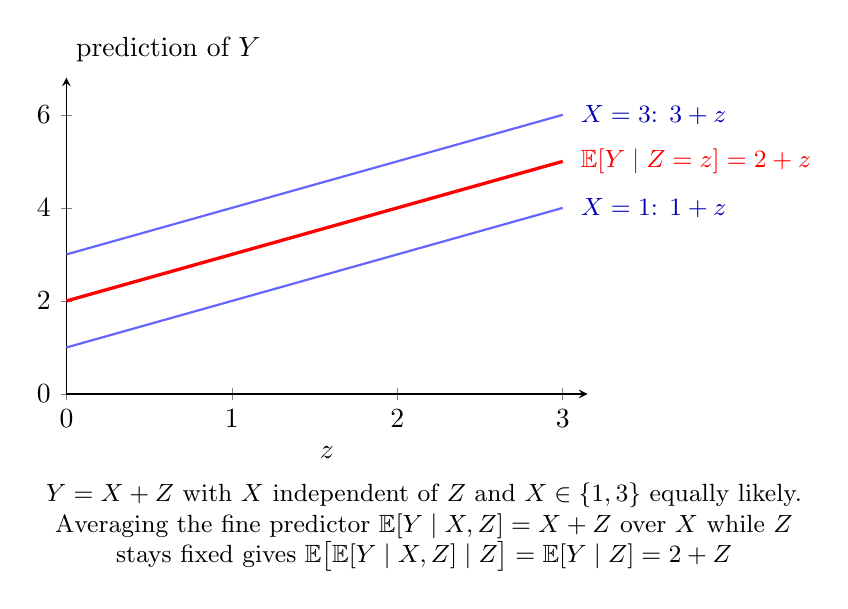
\begin{tikzpicture}
	\begin{axis}[
		axis lines=left, xmin=0, xmax=3.15, ymin=0, ymax=6.8,
		xtick={0,1,2,3}, ytick={0,2,4,6},
		xlabel={$z$}, ylabel={prediction of $Y$}, ylabel style={rotate=-90, anchor=south west, at={(axis description cs:0,1.02)}},
		width=8.2cm, height=5.6cm, clip=false
		]
		\addplot[blue!60, thick, domain=0:3] {1+x};
		\addplot[blue!60, thick, domain=0:3] {3+x};
		\addplot[red, very thick, domain=0:3] {2+x};
		\node[blue!70!black, anchor=west, font=\small] at (axis cs:3.05,4) {$X=1$: $1+z$};
		\node[blue!70!black, anchor=west, font=\small] at (axis cs:3.05,6) {$X=3$: $3+z$};
		\node[red, anchor=west, font=\small] at (axis cs:3.05,5) {$\mathbb{E}[Y\mid Z=z]=2+z$};
	\end{axis}
	\node[anchor=north, font=\small, align=flush center, text width=9.6cm] at ([yshift=-2pt]current axis.outer south) {$Y=X+Z$ with $X$ independent of $Z$ and $X\in\{1,3\}$ equally likely. Averaging the fine predictor $\mathbb{E}[Y\mid X,Z]=X+Z$ over $X$ while $Z$ stays fixed gives $\mathbb{E}\big[\mathbb{E}[Y\mid X,Z]\mid Z\big]=\mathbb{E}[Y\mid Z]=2+Z$};
\end{tikzpicture}
\end{document}
